\begin{frame}<1-3>[t]{新知探索}
\begin{campuscanvas}
% Source slide 5, objects 2; visible 2-3
\only<2-3|handout:1>{\node[anchor=north west,inner sep=0,text=black] at (70.000,150.000) {\begin{minipage}[t]{142.500mm}\raggedright\fontsize{13}{19.50}\selectfont 例如，单词 element 中出现的字母组成一个集合，$e$ 是这个集合的一个元素；太阳系的八大行星组成一个集合，地球是这个集合的一个元素；所有大于 $2$ 的素数组成一个集合，$7$ 是这个集合的一个元素；等等。\end{minipage}};}
% Source slide 5, objects 4; visible 3
\only<3|handout:1>{\node[anchor=north west,inner sep=0] at (300.000,390.000) {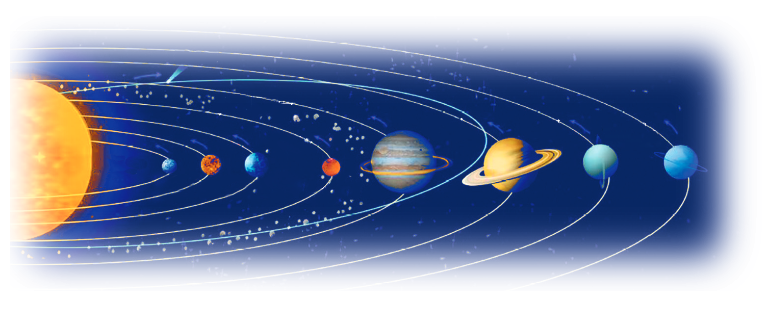
\includegraphics[width=85.000mm,height=35.375mm]{source-media/image12.png}};}
\end{campuscanvas}
\end{frame}
